\chapter{Realizace} \label{realizace}
% Popis implementace/realizace se zaměřením na nestandardní části řešení.
% A tady budu řešit jednotlivé Cisco příkazy - jak jsem na to přicházel, postupné problémy, moje implementace a odchylky.

Téměř všechny části systému obsahují tzv. debugovací mód, který vypisuje extra informace, co se právě děje nebo alepsoň přidává další vlastnost vhodnou pro ladění.

\section{Komunikační vrstva}
Server má sám pro sebe vlastní vlákno ve kterém běží. Dále server vytvoří při startu pro všechny počítače nová vlákna, která poslouchají na portu o~jedna větším než předchozí počítač (první počítač začíná na portu předaným jako parametr při startu serveru). Tyto vlákna se chovají zase jako servery. Když se uživatel připojí na libovolný počítač, tak se vytvoří další vlákno pro obsluhu tohoto klienta. Výhodou tohoto řešení je, že je možné se připojit na kterýkoliv počítač kolikrát potřebujeme. Je to tedy přesně tak, jako bychom se připojovali na reálné Cisco či linux např. přes protokol ssh\footnote{Secure Shell - zabezpečený komunikační protokol (v~současné době náhrada telnetu)} či telnet.

\begin{figure}[h]
\begin{center}
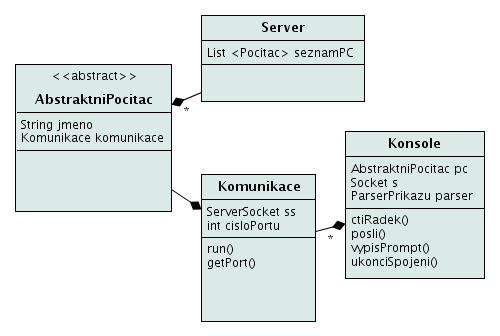
\includegraphics[width=9cm]{figures/uml_sit}
\caption{UML návrh komunikační části}
\label{uml:sit}
\end{center}
\end{figure}

Na obrázku \ref{uml:sit} je znázorněna komunikační část pomocí UML\footnote{Unified Modeling Language, UML je v~softwarovém inženýrství grafický jazyk pro vizualizaci, specifikaci, navrhování a dokumentaci programových systémů.\cite{wiki:uml}} diagramu. Každý počítač má objekt \verb|Komunikace|, ta čeká na připojení nového klienta. Když klient vyšle požadavek o~nové spojení, tak se vytvoří \verb|Konsole|, která tohoto klienta bude obsluhovat. Při odpojení klienta \verb|Konsole| zaniká, protože její přítomnost už není potřeba. \verb|Komunikace| se tedy chová jako server, který vytváří klienty - \verb|Konsole|.

%------------------------------------------------------------------------------

\section{Aplikační vrstva}
Předkem všech tříd systému na aplikační vrstvě je \verb|Abstraktni|, která zastřešuje převážně statické funkce např. \verb|zaokrouhli| (na tři desetinná místa), \verb|cekej| (metoda pro uspání vlákna, užitečná při výpisech Cisco IOS) a další. Od \verb|Abstraktni| dědí abstraktní \verb|ParserPrikazu|, který seskupuje všechny parsery příkazů (v~současné době pro linux a Cisco IOS). Společný předek linux a cisco příkazů je \verb|AbtraktniPrikaz|, z~kterého dědí linuxové příkazy kolegy a hlavně \verb|CiscoPrikaz|, který ještě přidává užitečné metody speciálně pro cisco příkazy. Viz obrázek \ref{uml:abstraktni}.

\begin{figure}[h]
\begin{center}
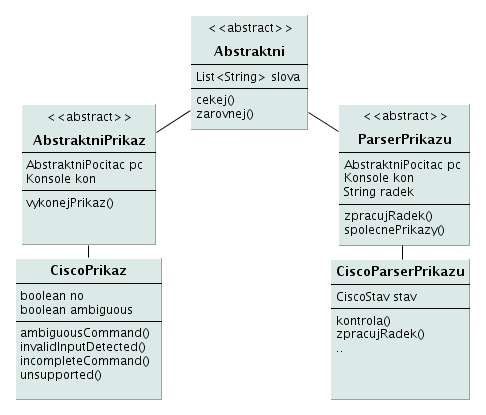
\includegraphics[width=9cm]{figures/uml_abtraktni.png}
\caption{Třídní model předků}
\label{uml:abstraktni}
\end{center}
\end{figure}

\subsection{Vyhodnocování příkazů}
Když uživatel zadá příkaz a ukončí ho znakem nového řádku (klávesa Enter, znak \verb|\n|), tak se ve třídě \verb|Konzole| zavolá metoda \verb|zpracujRadek()|. Tuto metodu vlastní abstraktní \verb|ParserPrikazu|, který je v~mém případe implementován jako \verb|CiscoParserPrikazu|\footnote{LinuxParser příkazů má na starosti kolega. Pro jiné typy počítačů je nutno implementovat parser vlastní.}. Ten se stará o~zpracování poslané řádky a podle toho volá různé Cisco příkazy, které tvoří IOS, nebo jiné servisní (obslužné) příkazy.

\subsection{Datové struktury jádra}
Datové struktury pro počítačovou síť byly vytvářeny ve spolupráci s~kolegou. \verb|CiscoPocitac| je má práce, třídy \verb|IpAdresa| a \verb|SitoveRozhrani| obsahují metody ode mne i od kolegy. Vlastnictví je blíže popsáno u~jednotlivých metod.

\begin{figure}[h]
\begin{center}
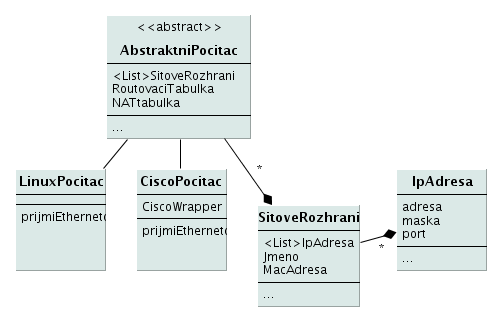
\includegraphics[width=10cm]{figures/uml_class}
\caption{Zjednodušený diagram tříd}
\label{uml:class}
\end{center}
\end{figure}


\subsubsection{Síťové rozhraní}
Datová struktura pro síťové rozhraní je ve své podstatě jednoduchá. Obsahuje jméno, seznam IP adres přiřazených k~tomuto rozhraní, MAC\footnote{MAC - Media Access Control, je fyzická adresa, kterou používá 2. (spojová) vrstva ISO/OSI modelu} adresu a stav.

Systémem je oficiálně podporována pouze jedna IP adresa per rozhraní, více adres si ale vyžádal překlad adres. MAC adresa je v~tomto systému spíše pro větší přiblížení skutečnému rozhraní, protože ARP\footnote{\uv{\textit{Address Resolution Protocol se v~počítačových sítích s~IP protokolem používá k~získání ethernetové MAC adresy sousedního stroje z~jeho IP adresy. Používá se v~situaci, kdy je třeba odeslat IP datagram na adresu ležící ve stejné podsíti jako odesilatel. Data se tedy mají poslat přímo adresátovi, u~něhož však odesilatel zná pouze IP adresu. Pro odeslání prostřednictvím např. Ethernetu ale potřebuje znát cílovou ethernetovou adresu.}}\cite{wiki:arp}} protokol v~této aplikaci přímo implementován. Systém obsahuje pouze několik pravidel, které byly nutné pro rozhodování zda přijmout či nepřijmout příchozí paket. Dále rozhraní obsahuje indikátor stavu, ve kterém se nachází - zapnuté/vypnuté. Rozhraní cisca jsou ve výchozím stavu vypnutá.

\newpage

\subsubsection{IP adresa}
\verb|IpAdresa| je mnohem složitější třída než rozhraní i když obsahuje pouze tři čísla reprezentující adresu, masku a port. Složitost je dána tím, že tato třída obsahuje přes 40 obslužných metod, které pokrývají veškerou práci, kterou je potřeba vykonávat (výpočet čísla sítě a broadcastu, kontrolní metody pro ověřování správnosti IP adresy, ..).

%------------------------------------------------------------------------------

\section{Parser Cisco}

\subsection{Cisco IOS}
Cisco IOS je operační systém, který se nachází na drtivé většině směrovačů firmy Cisco Systems. IOS obsahuje pouze ovládání přes příkazový řádek (CLI\footnote{Command Line Interface}). IOS obsahuje tzv. zkracování příkazů, které zefektivňuje práci s~celým systémem. Celé to funguje tak, že když uživatelův příkaz lze doplnit na jeden jedinečný příkaz (samotné doplnění přes klávesu \verb|TAB|), tak to takový příkaz hned zavolá. Například příkaz \verb|sh run| lze jednoznačně doplnit na \verb|show running-config|, ale kratší \verb|sh ru| už ne:
\begin{verbatim}
Router#sh ru?
rudpv1  running-config
\end{verbatim} 

IOS tvoří několik stavů, např.:
\begin{itemize}
 \item uživatelský mód
 \item privilegovaný mód
 \item konfigurační mód - zde se nastavují volby, které ovlivní celý systém
 \item konfigurace rozhraní - konfigurace jednoho určitého rozhraní
\end{itemize}

\begin{figure}[h]
\begin{center}

\includegraphics[width=13cm]{figures/ios.png}
\caption{Přehled základních módů Cisco IOS \cite{wiki:ios}}
\label{fig:ios}
\end{center}
\end{figure}

Na obrázku \ref{fig:ios} jsou zobrazeny důležité stavy IOS a přechody mezi nimi. 

%------------------------------------------------------------------------------

\subsubsection{Uživatelský mód}
Uživatelský mód (USER MODE) je výchozí (startovací) mód. Tento mód je značně limitovaný a dovoluje použití čistě read-only příkazů (tj. takových, které nezmění konfiguraci). Přesto má tento mód svoje opodstatnění, dovoluje např. vypsat směrovací tabulku (\verb|show ip route|) či použít příkazy \verb|ping| nebo \verb|traceroute|. Do privilegovaného režimu se lze přepnout příkazem \verb|enable|.

\subsubsection{Privilegovaný mód}
Privilegovaný mód (PRIVILEGED MODE) nebo také \uv{administrátorský} mód je podobný linuxovému \verb|root| účtu. Tento mód je výchozím bodem pro vstup do ostatních módů. Pro návrat zpět do uživatelského režimu existuje příkaz \verb|disable|. Příkaz \verb|configure| způsobí přepnutí do dalšího konfiguračního módu. Privilegovaný mód umožňuje vypsat veškeré informace o~aktuální konfiguraci systému, např.:
\begin{itemize}
 \item \verb|show running-config| - shrnutí aktuální konfigurace
 \item \verb|show ip route| - výpis směrovací tabulky
 \item \verb|show ip nat translations| - výpis dynamických záznamů v~NAT tabulce
\end{itemize}
Není důvod, proč by v~tomto stavu nefungovaly příkazy \verb|ping| a \verb|traceroute|.

\subsubsection{Konfigurační mód}
Konfigurační mód (CONFIG MODE) je jeden z~nejdůležitějších, protože umožňuje konfiguraci směrovacích záznamů (\verb|ip route|), přístupových seznamů pro potřeby překladu adres (\verb|access-list|), pooly IP adres (\verb|ip nat pool|) a výběr rozhraní pro přechod do stavu konfigurace rozhraní (\verb|interface|).

\subsubsection{Konfigurace rozhraní} \label{configif}
V~tomto módu lze nastavovat IP adresy na aktuálně vybrané rozhraní, nastavovat příznaky pro veřejné a soukromé rozhraní pro NAT (\verb|nat inside|, \verb|nat outside|) nebo také zapínat či vypínat rozhraní. Pro přechod ze všech konfiguračních módů do privilegovaného stačí napsat příkaz \verb|end| nebo jen stisknout klávesovou zkratku \verb|Ctrl+Z|.

%------------------------------------------------------------------------------

\subsection{Implementace Cisco IOS}
Cisco IOS obsahuje desítky příkazů z~nichž každý může mít až stovky variací. Proto jsem implementoval pouze úzkou část příkazů, která je potřebná pro splnění zadání této práce. Nejdůležitější funkcí parseru je rozpoznávání zkrácených příkazů. Na skutečném Ciscu se opravdu procházejí všechny možnosti, které mohou v~daném stavu nastat, a podle nich probíhá vyhodnocování. V~mé implementaci ale mám pouze část příkazů, takže jsem to musel vyřešit jiným způsobem. Pro každé slovo (část příkazu) si \verb|CiscoParserPrikazu| drží počet písmen, který je potřeba k~jednoznačnému určení příkazu. Tato čísla jsem \uv{naměřil} na školních ciscách v~březnu 2010. Zajímavé je, že už o~2 měsíce později jsem objevil drobné změny. Čísla se mohou měnit s~různými verzemi Cisco IOS. To bych ale neviděl jako zásadní problém. Většina studentů (alespoň dle mé zkušenosti) stejně píše celé příkazy a zkrácené verze nepoužívá, protože je zpravidla nezná.

Vyhodnocování příkazů zajišťuje metoda \verb|kontrola(command, cmd)|. Parametr \verb|command| je celý příkaz, na který by se to mohlo eventuálně doplnit, a \verb|cmd| je příkaz poslaný od uživatele. Nejdříve se zjistí počet znaků, který je potřeba pro jednoznačné doplnění na příkaz \verb|command|. Po té se zkontroluje požadovaný počet znaků a také jestli zkrácený příkaz odpovídá doplněnému. A~takto to vypadá v~kódu:

\begin{verbatim}
if (cmd.length() >= i && command.startsWith(cmd)) {
    // i..požadovaný počet znaků 
    // lze doplnit na jeden jedinečný příkaz
    return true;
}
if (command.startsWith(cmd)) {
    // vypsat amiguous command
    nepokracovat = true;
}
\end{verbatim}

Jednotlivé příkazy Cisco IOS jsou implementovány v~samostatných třídách. Třída \\\verb|CiscoParserPrikazu| zajišťuje přechody mezi stavy (módy) a navíc se stará o \uv{nahazování} rozhraní. Přepnutí stavu rozhraní je natolik triviální, že se by se nevyplatilo mít pro to zvláštní třídu. 

\paragraph{}
Ladící mód zjednodušuje testování parseru a přidává tyto funkce:
\begin{itemize}
 \item klávesa \verb|Enter| funguje jako přechod z~uživatelského do privilegovaného módu
 \item použití příkazů z~jiných módů v~privilegovaném módu - navíc např. \verb| ip route|, \\\verb|ip nat pool inside|, \verb|access-list|, ..
 \item extra výpis dynamických záznamů v~natovací tabulce
 \item výpis \verb|show running-config| je pro přehlednost zkrácen
 \item možnost testování routovací tabulky přes linuxový příkaz \verb|route|
 \item používání linuxového příkazu \verb|ifconfig|
\end{itemize}
Použití těchto funkcí je vhodné spíše pro ladění programu do budoucna než pro běh v~\uv{ostrém} provozu. Tento mód je ve výchozím stavu vypnut.

%------------------------------------------------------------------------------

\subsection{Odchylky v~implementaci}
Má implementace Cisco IOS má navíc pár příkazů, které jsou potřeba pro ovládání systému. Jak už jsem se zmiňoval v~kapitole \ref{kap:podobnost} je zde navíc \verb|help| a \verb|help_en| pro výpis nápovědy. Příkaz \verb|kill| přijde vhod, když uživatel chce ihned vypnout aplikaci a nechce projít přes několik stavů příkazem \verb|exit|. Další servisní příkaz je \verb|save| nebo také \verb|uloz|, který zapíše aktuální konfiguraci všech počítačů do konfiguračního souboru, se kterým byl spuštěn nebo který byl předán jako parametr. Dále lze využít velmi jednoduchý příkaz \verb|?| (otazník), který vypíše seznam dostupných příkazů v~aktuálním stavu.

Na skutečném Ciscu funguje kombinace kláves \verb|Ctrl+Z| pro přechod do privilegovaného módu. Ale kvůli použití programu \verb|rlwrap| je systém limitován. Omezení spočívá v~tom, že \verb|rlwrap| přepošle signál operačnímu systému a ten pozastaví tento proces. Proces lze obnovit příkazem fg (na OS Linux), bohužel klientský program \verb|telnet| neumí po pozastavení obnovit svoji funkčnost a přestává posílat vstup na standartní výstup. Je tedy už nepoužitelný a pro tyto přídady existuje příkaz \verb|kill|, který ukončí tento rozbitý proces, aby se klient mohl připojit znova. Lépe je na tom klávesová zkratka \verb|Ctrl+C|, která pouze ukončuje (signál SIG\_INT) daný proces a tedy funguje bez problému. 

Program \verb|rlwrap| je ale šířen jako balíček pod programem \verb|cygwin| v~zastaralé verzi\footnote{stav z~18.5.2010}, která neumožňuje přeposílání signálů, takže při stisku \verb|Ctrl+C| i \verb|Ctrl+Z| přestane \verb|telnet| klient vypisovat na standartní výstup a nezbývá než použít \verb|kill|. Toto platí pouze na OS Windows, pro linux jsou dostupné nejnovější balíčky v repozitářích každé distribuce.



